\documentclass[12pt]{ito}
% Paquetes de prueba
\usepackage{lipsum}

\autor{NOMBRE DEL AUTOR}
\titulo{TÍTULO DEL TRABAJO}
\director{NOMBRE DEL DIRECTOR}
\codirector{NOMBRE DEL CODIRECTOR}
\keywords{SOME, KEY, WORDS}
\palabras{ALGUNAS, PALABRAS, CLAVE}

\graphicspath{ {imagenes/} }
\addbibresource{referencias.bib}

\includeonly{
    contenido/preambulo/resumen,
    contenido/preambulo/abstract,
    contenido/preambulo/introduccion,
    contenido/preambulo/planteamiento,
    contenido/preambulo/justificacion,
    contenido/preambulo/hipotesis,
    contenido/preambulo/objetivos,
    contenido/capitulos/antecedentes,
    contenido/capitulos/estado,
    contenido/capitulos/metodologia,
    contenido/capitulos/resultados,
    contenido/epilogo/conclusiones,
    contenido/epilogo/recomendaciones,
    contenido/epilogo/productos,
    contenido/epilogo/anexos
}

\begin{document}

\maketitle

\tableofcontents
\listoffigures
\listoftables

% Preambulo
\prechapter{RESUMEN}

\lipsum[1-2]

\makeatletter
\textbf{Palabras Clave:} \@palabras
\makeatother
% \lipsum[2-4]
\prechapter{ABSTRACT}

\lipsum[1-2]

\makeatletter
\textbf{Keywords:} \@keywords
\makeatother
\prechapter{INTRODUCCIÓN}

\lipsum[1-2]
\prechapter{PLANTEAMIENTO DEL PROBLEMA}

\lipsum[1-2]
\prechapter{JUSTIFICACIÓN}

\lipsum[1-2]


\lipsum[1-2]


\lipsum[1-1]

\section*{OBJETIVOS ESPECÍFICOS}
\addcontentsline{toc}{section}{OBJETIVOS ESPECÍFICOS}

\lipsum[1-1]

% Capitulos
\chapter{ANTECEDENTES}

\lipsum[1-1] \parencite{knuth:1984}

\begin{figure}[H]
    \centering
    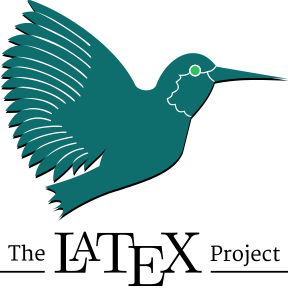
\includegraphics[width=0.5\textwidth,height=0.5\textwidth]{latex_project}
    \caption{Mi figura uno}\label{fig:fig1}
\end{figure}
\chapter{ESTADO DEL ARTE}

\lipsum[1-3] \parencite{latex:companion}

\chapter{METODOLOGÍA}

\lipsum[1-1] \parencite{latex2e}

En la \vref{tab:tabla1} podemos observar un ejemplo de tabla.

\begin{table}[H]
	\centering
	\caption{Mi tabla}\label{tab:tabla1}
	\begin{tabular}{@{}llr@{}}
		\toprule
		\multicolumn{2}{c}{Item} &                          \\ \cmidrule(r){1-2}
		Animal                   & Description & Price (\$) \\ \midrule
		Gnat                     & per gram    & 13.65      \\
		                         & each        & 0.01       \\
		Gnu                      & stuffed     & 92.50      \\
		Emu                      & stuffed     & 33.33      \\
		Armadillo                & frozen      & 8.99       \\ \bottomrule
	\end{tabular}
\end{table}

Este es un ejemplo de una referencia \cref{noexiste} y de una cita\autocite{noexiste} no encontradas.
\chapter{RESULTADOS}

\lipsum[1-1] \cite{texbook}

\begin{figure}[H]
    \centering
    
\includegraphics[width=\textwidth,height=0.5\textwidth]{overleaf}
    \caption{Mi figura dos}\label{fig:fig2}
\end{figure}



% Epilogo
\prechapter{CONCLUSIONES}

\lipsum[1-2] \parencite{lesk:1977}

\prechapter{RECOMENDACIONES}

\lipsum[1-2]

\printbibliography[title={REFERENCIAS BIBLIOGRÁFICAS},heading=bibintoc]

\prechapter{PRODUCTOS ACADÉMICOS}

\lipsum[1-1]
\lipsum[1-3]



\end{document}